\documentclass{article}
\usepackage{tikz,amsmath}
\title{CSC 320 Assignment 3}
\author{Oliver Tonnesen\\V00885732}
\date{March 18, 2019}
\begin{document}
\maketitle
\renewcommand{\thesubsection}{\thesection.\alph{subsection}}

\section{} % Section 1
Yes. We provide constructions for TMs deciding the three languages. Let $M_1$
be a decider for $L_1$, and $M_2$ be a decide for $L_2$.
\newline
\newline
\underline{Concatenation ($L_1\circ L_2$)}: Our Nondeterministic Turing
Machine operates as follows:
\newline
\newline
Run like $M_1$ on the input. Whenever $M_1$ would enter an accepting state,
branch and run like $M_2$ on the remainder of the input. Accept when any branch
of computation finishes in an accepting state of $M_2$, reject otherwise.
\newline
\newline
\underline{Intersection ($L_1\cap L_2$)}: Our Turing Machine operates as
follows:
\newline
\newline
Run like $M_1$ on the input and reject if $M_1$ rejects. Then, run like $M_2$
on the input and accept if $M_2$ accepts, and reject if $M_2$ rejects.
\newline
\newline
\underline{Complement ($\overline{L_1}$)}: Our Turing Machine operates as
follows:
\newline
\newline
Run like $M_1$ on the input. Accept if $M_1$ rejects, reject if $M_1$ accepts.

\section{} % Section 2
We will encode the following Turing Machine:
\newline
\newline
\begin{minipage}{\textwidth}
\begin{center}
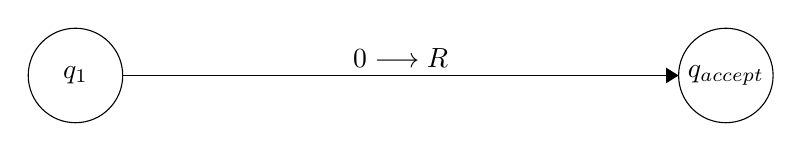
\begin{tikzpicture}[scale=0.2]
\tikzstyle{every node}+=[inner sep=0pt]
\draw [black] (18.7,-29.1) circle (3);
\draw (18.7,-29.1) node {$q_1$};
\draw [black] (60,-29.1) circle (3);
\draw (60,-29.1) node {$q_{accept}$};
\draw [black] (21.7,-29.1) -- (57,-29.1);
\fill [black] (57,-29.1) -- (56.2,-28.6) -- (56.2,-29.6);
\draw (39.35,-28.6) node [above] {$0\longrightarrow R$};
\end{tikzpicture}
\end{center}

\end{minipage}
\newline
\newline
We assume that $\Sigma=\{0,1\}$. Also recall that $q_{accept}$ becomes $q_2$
for the purposes of our encoding.
\newline
\newline
Let $X_1=0,X_2=1$. Then our transition function contains the following:
\[\delta(q_1,X_1)=(q_2,X_1,D_2)\]
and we encode it as:
\[0^110^110^210^110^2=01010010100\]

\section{} % Section 3
Assume for a contradiction that $L$ is decidable. Then there exists a Turing
Machine that decides $L$, call it $R$.
\newline
\newline
For any $\langle M,w\rangle$, $M_1$ runs as follows:
\begin{itemize}
	\item Run like $M$ on input $w$ and write a \$ when and only when $M$
		accepts $w$
\end{itemize}
We construct $V$ to run on $\langle M,w\rangle$ as follows:
\begin{itemize}
	\item Use $\langle M,w\rangle$ to output $\langle M_1\rangle$
	\item Run $R$ on $\langle M_1\rangle$
	\item If $R$ accepts, accept. If $R$ rejects, reject.
\end{itemize}
Thus $V$ decides $A_{TM}$, and so our assumption that $L$ is decidable was
false.
\newline
\newline
Assuming we are able to choose the encoding of our Turing Machine, it does not
matter what symbol we choose to take the place of \$. That is, if we were to
choose 1, for example, we could simply modify the Turing Machine to use 2
whenever it would otherwise use 1, and use 1 only in the specific case where we
need it.

\section{} % Section 4
$M$ has a finite number of states, so we can simply construct a Turing Machine
to simulate $M$ until it either writes a symbol to its tape, or returns to a
state that has already been visited. We know that $M$'s behaviour at a
particular state will not change if its tape has not been changed. So our
Turing Machine will have to simulate at most $M$ states of $M$'s computation
before it is able to confirm whether or not $M$ ever writes a symbol to its
tape.

\section{} % Section 5
If $\langle M\rangle$ is in $\overline{E_{TM}}$, then there exists a string $w$
accepted by $M$. Thus our Nondeterministic Turing Machine can simply run like
$M$ on every binary string and accept when one branch of computation ends in
the accept state. Clearly $w$ is one of the binary strings, so our constructed
Nondeterministic Turing Machine always accepts if $L(M)\neq\emptyset$, and
$\overline{E_{TM}}$ is thus recognizable.

\section{} % Section 6
We know that $E_{TM}$ is undecidable, so since $\overline{E_{TM}}$ is
recognizable, $E_{TM}$ clearly cannot be recognizable.
\newline
\newline
We define the following computable function:
\begin{align*}
	f:\Sigma^*&\longrightarrow\Sigma^*\\
	\langle M\rangle&\longmapsto\langle M,M\rangle
\end{align*}
We know that
\[L(M)\cap L(M)=L(M)\]
so it must be the case that
\[L(M)=\emptyset\Longleftrightarrow L(M)\cap L(M)=\emptyset\]
In other words,
\[\langle M\rangle\in E_{TM}\Longleftrightarrow\langle M,M\rangle\in\{\langle M_1,M_2\rangle\mid L(M_1)\cap L(M_2)=\emptyset\}\]
Thus we have given the reduction
\[E_{TM}\le_M\{\langle M_1,M_2\rangle\mid L(M_1)\cap L(M_2)=\emptyset\}\]
We know that $E_{TM}$ is not recognizable, and so
$\{\langle M_1,M_2\rangle\mid L(M_1)\cap L(M_2)=\emptyset\}$ is also not
recognizable.
\end{document}
